\section{Discussions}\label{chapter-ML-section-discussion}
Les effets
de l'empilement,
de la reconstruction des particules,
des faux taus hadroniques,
de la séparation des canaux et
de l'intervalle de masse
sur les prédictions de masse
sont discutées ci-après.
Lors de notre étude, ces effets ont été observés en parallèle de l'exploration des hyper-paramètres présentée en section~\ref{chapter-ML-section-hyperparameters} avec des modèles divers.
À des fins de cohérence dans la comparaison des effets,
nous utilisons ici le modèle B sélectionné précédemment comme référence.
\subsection{Effet de l'empilement}
\def\Bnpu{$\text{B}^\text{0PU}$}
Dans les travaux de \citeauthor{BARTSCHI201929}~\cite{BARTSCHI201929},
l'empilement (PU, \emph{Pile-Up}) n'est pas considéré.
Nous avons donc souhaité déterminer l'effet du PU sur les prédictions de notre modèle.
Pour cela, les mêmes événements que ceux décrits en section~\ref{chapter-ML-section-evt_gen} ont été générés sans PU.
Un DNN, noté \Bnpu, est entraîné sur ces événements sans PU.
Les hyper-paramètres de \Bnpu\ sont ceux de B, à l'exception des variables d'entrées auxquelles \Npu\ est retiré, car $\Npu=0$ pour tous les événements sans PU.
La réponse de \Bnpu\ sur les événements de test sans PU est représentée sur la figure~\ref{subfig-reponse_model_PU_00}.
La réponse du modèle est de l'ordre de 1 pour $m_{\higgsML}$ entre \SI{80}{\GeV} et \SI{600}{\GeV} avec une résolution à $\pm1\sigma$ de l'ordre de \SI{20}{\%} à basse masse et \SI{10}{\%} à haute masse.
\begin{figure}[h]
\centering

\subcaptionbox{Réponse de \Bnpu\ sur les événements sans PU.\label{subfig-reponse_model_PU_00}}[.45\textwidth]
{\includegraphics[width=.45\textwidth]{\PhDthesisdir/plots_and_images/my_plots/ML/from_ML_plots/DNNs_for_discussion/PU/trained_wo_PU_wo_Npu/test_wo_PU/model_response-NN-activation-softplus-batch_size-2048-mape-Adam-gu-inclusive-3-layers-1000-neurons.pdf}\vspace{-.5\baselineskip}}
\hfill
\subcaptionbox{Réponse de \Bnpu\ sur les événements avec PU.\label{subfig-reponse_model_PU_01}}[.45\textwidth]
{\includegraphics[width=.45\textwidth]{\PhDthesisdir/plots_and_images/my_plots/ML/from_ML_plots/DNNs_for_discussion/PU/trained_wo_PU_wo_Npu/test_on_PU/model_response-NN-activation-softplus-batch_size-2048-mape-Adam-gu-inclusive-3-layers-1000-neurons.pdf}\vspace{-.5\baselineskip}}

\caption{Réponses du modèle \Bnpu\ sur les événements sans et avec PU.}
\label{fig-reponse_model_0PU}
\end{figure}
\par
Cependant, la réponse de \Bnpu\ est dégradée sur des événements contenant du PU, figure~\ref{subfig-reponse_model_PU_01}.
La réponse médiane se situe en effet à \num{1.2} à $m_{\higgsML}=\SI{100}{\GeV}$ et diminue à \num{0.9} à $m_{\higgsML}=\SI{800}{\GeV}$ contre \num{1.05} et \num{0.9} sans PU respectivement.
La résolution relative à basse masse est de l'ordre de \SI{30}{\%}.
Plus $m_{\higgsML}$ est faible,
plus basse est l'énergie portée par $L_1$ et $L_2$, issue de la masse de \higgsML.
Alors, les particules du PU sont compétitives, en termes de propriétés cinématiques, avec $L_1$ et $L_2$.
Lors de la sélection des événements et de la construction du \emph{dilepton} présentée au chapitre~\refChHTT,
il est ainsi possible que les particules utilisées en tant que $L_1$ ou $L_2$ soient en réalité issues du PU et non de la désintégration de \higgsML.
Plus $m_{\higgsML}$ augmente, moins le PU est compétitif, d'où l'atténuation de l'effet sur la réponse observée du modèle.
Il est donc primordial d'inclure le PU dans l'entraînement dans l'optique d'une utilisation de nos modèles dans les analyses de CMS.
\par
La réponse du modèle B, entraîné avec PU, peut être comparée
dans le cas d'événements sans PU, figure~\ref{subfig-reponse_model_PU_10},
au cas d'événements avec PU, figure~\ref{subfig-reponse_model_PU_11} (identique à~\ref{subfig-reponse_model_B}).
Le profil de PU utilisé pour générer les événements d'entraînement est celui de l'année 2017.
Or, il apparaît que le modèle B est peu sensible au retrait du PU, les réponses étant similaires sur les figure~\ref{subfig-reponse_model_PU_10} et~\ref{subfig-reponse_model_PU_11}.
L'utilisation de B sur des événements dont le profil de PU est légèrement différent de celui de l'année 2017,
comme c'est le cas pour les autres années du Run~II (2016, 2018)
est ainsi directement envisageable.
\begin{figure}[h]
\centering

\subcaptionbox{Réponse de B sur les événements sans PU.\label{subfig-reponse_model_PU_10}}[.45\textwidth]
{\includegraphics[width=.45\textwidth]{\PhDthesisdir/plots_and_images/my_plots/ML/from_ML_plots/DNNs_for_discussion/PU/trained_on_PU/test_wo_PU/model_response-NN-ADAM_glorot_uniform-activation-softplus-batch_size-2048-mape-Adadelta-u-inclusive-3-layers-1000-neurons.pdf}\vspace{-.5\baselineskip}}
\hfill
\subcaptionbox{Réponse de B sur les événements avec PU.\label{subfig-reponse_model_PU_11}}[.45\textwidth]
{\includegraphics[width=.45\textwidth]{\PhDthesisdir/plots_and_images/my_plots/ML/from_ML_plots/trained_NNs_FastSim/DeepTau-inclusive/PuppiMET_with_METcov_j1j2jr_Nnu_Npu/model_response-NN-ADAM_glorot_uniform-activation-softplus-batch_size-2048-mape-Adadelta-u-inclusive-3-layers-1000-neurons.pdf}\vspace{-.5\baselineskip}}

\caption{Réponses du modèle B sur les événements sans et avec PU.}
\label{fig-reponse_model_1PU}
\end{figure}
\subsection{Effet de la reconstruction}
\def\Bgenleg{$\text{B}^\text{gen}$}
La reconstruction des particules est présentée dans le chapitre~\refChLHCCMS.
Son effet peut être caractérisé par l'étude du modèle \Bgenleg,
ayant les mêmes hyper-paramètres que B mais entraîné en utilisant les objets générées au lieu des ceux reconstruits pour $L_1$, $L_2$ et \MET, \ie\ pour les trois objets physiques issus de la désintégration des leptons tau (deux parties visibles et \MET\ pour les neutrinos).
En particulier, les valeurs de $\pT^{L_1}$, $\pT^{L_2}$ et \MET\ correspondent exactement à la réalité physique.

\begin{figure}[h]
\centering

\subcaptionbox{Réponse de \Bgenleg\ dans le cas d'une reconstruction parfaite.\label{subfig-reponse_model_GENleg_10}}[.45\textwidth]
{\includegraphics[width=.45\textwidth]{\PhDthesisdir/plots_and_images/my_plots/ML/from_ML_plots/DNNs_for_discussion/Reco_effect/GENleg_with_METcov_j1j2jr_Nnu_Npu/model_response-NN-activation-softplus-batch_size-2048-mape-Adam-gu-inclusive-3-layers-1000-neurons.pdf}\vspace{-.5\baselineskip}}
\hfill
\subcaptionbox{Réponse de \Bgenleg\ dans le cas d'une reconstruction réelle.\label{subfig-reponse_model_GENleg_11}}[.45\textwidth]
{\includegraphics[width=.45\textwidth]{\PhDthesisdir/plots_and_images/my_plots/ML/from_ML_plots/DNNs_for_discussion/Reco_effect/GENleg_with_METcov_j1j2jr_Nnu_Npu/test_on_reco/model_response-NN-activation-softplus-batch_size-2048-mape-Adam-gu-inclusive-3-layers-1000-neurons.pdf}\vspace{-.5\baselineskip}}

\caption{Réponses du modèle \Bgenleg\ dans le cas d'une reconstruction des particules parfaite et réelle.}
\label{fig-reponse_model_1GENleg}
\end{figure}

show trained/tested on gen tau, gen tau decays, reco tau decays (=real), see fig 3 from report 2021-01-11

the model understand the physics, now it has to deal with the reco resolution and fakes.

\subsection{Effet des faux taus hadroniques}

\subsection{Effet de la séparation des canaux}
not relevant (fig3 report  2021-01-21)


\subsection{Effet de l'intervalle de masse}
\subsubsection{Gamme de masse}

\subsubsection{Effet de bord}

use the custom loss with boundaries cuts (basically all the report 2021-02-04)

Follow report from 2021-02-04 but for section 3 : We saw that predictions come out too low, which already is a motivation to put larger weights on higher masses, i.e. to weight by truth. Choosing sqrt(truth) is of course just a guess then

extend up to 1TeV using the tails


\subsection{Modèle final}

\DEEPTAU

1 TeV

all inputs

activation softplus

loss mapesqrt\_b

opti Adam

glorot uniform

3 layers of 1000 neurons

show reponses and 2d histo
